\section{L'implementazione del database}
Nelle sezioni precedenti si è discusso delle proprietà
offerte dai diversi tipi di database e
delle necessità che il dominio impone sul sistema.
La scelta del database deriva quindi dall'incrocio di tutte queste condizioni,
individuando la tecnologia che meglio riesce a rispondere alle esigenze del progetto.
Ogni tipologia di database comporta un approccio differente alle informazioni,
implicando una strategia di salvataggio e manipolazione dei dati propria.
Le strutture che modellano le entità devono quindi
essere create per sfruttare nella maniera più efficiente possibile
i vantaggi offerti dalla tecnologia scelta.\\
\\
Una volta scelto il database e le strutture in base alla modalità
che più si addicono alle esigenze del progetto,
l'utilizzo di servizi in cloud comporta una maggiore attenzione anche
alle proprietà legate al mantenimento del servizio,
dalle quali derivano le proprietà di scalabilità e affidabilità.
La grande differenza tra i vari servizi sta nelle proprietà del server
incaricato di fornire il potere computazionale necessario per l’esecuzione.
L’architettura del server e la sua integrazione con la tecnologia del database
determinano infatti l’effettiva capacità di scalabilità del servizio.\\
\\
Si intende scalabilità verticale la capacità di aumentare le risorse
della stessa macchina in cui si esegue il codice.
La scalabilità verticale viene definita nel momento di creazione del servizio,
in cui si determinano le risorse da dedicare alla macchina che esegue il programma.
Trattandosi di macchine virtualizzate,
è sempre possibile in un secondo momento aumentare le prestazioni in caso di necessità.\\
\\
Per scalabilità orizzontale si intende invece la capacità di
delegare il carico di lavoro su più macchine, eventualmente coordinando le modifiche.
Questo permette una risposta alle richieste più resistente,
riducendo il rischio di colli di bottiglia che potrebbero venirsi a formare nell’utilizzo di un nodo singolo.
La scalabilità orizzontale richiede però l'implementazione
di tecnologie apposite integrate con il database che permettano l'esecuzione in nodi fisici differenti. \\
\\
Una volta individuata la tecnologia adatta e il livello di scalabilità desiderati,
è bene considerare le altre necessità o le opportunità aggiuntive generate
dalla presenza di un database nel progetto. \\
\\
L’alta disponibilità(HA) è la proprietà di garantire l’accesso al servizio nonostante i guasti.
Ad esempio, si può mantenere una macchina identica al server principale in grado di replicare il servizio,
spostando il carico in caso di guasto del server principale.
Si misura in “numero di nove”, ovvero la quantità di nove presenti
nella percentuale del tempo per il quale si garantisce la disponibilità del servizio.
I servizi offrono diverse qualità di HA, in base alle funzionalità desiderate.\\
\\
Alcuni servizi possono presentare offerte di backup
per riportare il server nello stesso stato di qualche momento precedente.
Questo permette il ripristino del sistema a un punto precedente
rispetto all'avvenimento di eventuali errori o guasti del sistema.\\
\subsection{La scelta del database}

Viste le necessità del progetto in ambito di scalabilità
e le caratteristiche del dominio,
si individua nei database documentali la tecnologia più adatta
per gestire la persistenza centrale dell'applicazione.\\
\\
I database documentali, facenti parte della categoria dei database non relazionali,
rappresentano un paradigma di gestione dei dati
che organizza le informazioni in documenti.
Ogni documento è un'unità autonoma che incapsula la descrizione di un'entità,
contenendo le sue proprietà.
Tali documenti sono logicamente raggruppati in collezioni.
All'interno di una collezione,
ciascun documento è univocamente identificato da un proprio identificativo,
garantendo l'accesso diretto e la manipolazione individuale.\\
\\
Un aspetto distintivo e strategicamente rilevante dei database documentali è
la loro intrinseca capacità di supportare la scalabilità orizzontale in modo nativo.
Data la natura dei documenti e il loro accoppiamento debole con gli altri elementi,
la separazione delle collezioni risulta particolarmente semplificata,
favorendo un partizionamento dei dati,  
essenziale per distribuire il database su diversi nodi fisici di archiviazione.
Questo vantaggio è fondamentale in architetture distribuite e ambienti ad alta intensità di dati.\\
\\
Un altro vantaggio derivato dall'utilizzo di un database non relazionale
è la propensione verso la denormalizzazione degli elementi del dominio, 
sia strutturale che logica.
La denormalizzazione consiste nel riportare le stesse proprietà degli elementi in più collezioni, 
riducendo così, se correttamente ottimizzata, 
il numero di join o richieste al database necessario per soddisfare le richieste.
Infatti, vista la riduzione di efficienza nell'incrocio tra entità, 
dovuta a una difficoltà intrinseca nell'ottimizzare le join tra documenti,
si propende, invece che a incrociare i dati, a duplicarli sui i vari documenti.
Le operazioni di join sono così agevolate,
in quanto possono essere ottimizzate per 
far risiedere la risorsa voluta all'interno dello stesso documento o nella stessa partizione dell'elemento di partenza, 
minimizzando la necessità di operazioni di giunzione di tabelle o di lettura tra nodi distinti.
Questo permette di aggregare i dati attorno agli elementi chiave su cui vertono le richieste,
favorendo la divisione dei dati anche in caso di relazioni complesse.\\
\\
La denormalizzazione comporta però intrinsecamente
alcune sfide a livello di consistenza dei dati,
in particolare per le operazioni di modifica che coinvolgono informazioni duplicate.
Infatti, pur se si modificasse atomicamente il documento direttamente coinvolto dalla modifica,
bisognerebbe comunque aggiornare tutte le altre parti che includono quella proprietà.
Oltre a dover progettare l'applicazione affinché sia resiliente all'inconsistenza temporanea,
ad esempio mostrando dati "vecchi" per un breve periodo prima che le modifiche vengano propagate, 
o implementando logiche di compensazione che possano correggere eventuali discrepanze,
è quindi necessario implementare la logica per garantire che la modifica venga propagata correttamente.
Esistono diverse strategie gestire le informazioni duplicate in modo efficace e mitigarne l'impatto. 
Una delle soluzioni avviene tramite trigger a livello di database, 
che scatena la chiamata che corregge poi i dati ove necessario.
Le code di messaggistica prevedono invece un orchestratore per la distribuzione degli aggiornamenti, 
che riceve notifiche delle variazioni e le elabora per poi applicare le modifiche.
Un'altra tecnica è l'applicazione di servizi in background che periodicamente scansionano e sincronizzano i dati. 
Infine, si possono adottare timestamp o numeri di versione su ciascun documento o campo denormalizzato,
permettendo alle applicazioni di determinare la versione più recente di un dato, 
risolvendo i conflitti quando si presentano aggiornamenti concorrenti o ritardati.\\
\\
Implementando automaticamente e nativamente la scalabilità orizzontale,
il database relazionale ci permette quindi di gestire con efficienza
l'incremento dei volumi di dati e dei carichi di lavoro senza interventi complessi.
Fornisce inoltre un supporto diretto all'esigenza dell'architettura
riguardo alla necessita di letture performanti
da entrambi i lati di relazioni molti-a-molti:
attraverso il partizionamento strategico,
i dati correlati possono essere collocati in partizioni vicine
per ottimizzare le letture da entrambi i lati della relazione.
Infine, un'attenta progettazione del modello di dati,
che include una denormalizzazione strategica e l'utilizzo degli indici,
garantirà un tempo di recupero ridotto per le informazioni,
massimizzando la reattività del sistema e l'efficienza complessiva.\\
\\
Un confronto con il paradigma relazionale evidenzia le ragioni della sua esclusione per le esigenze del nostro progetto.
Sebbene i database relazionali siano soluzioni consolidate per la gestione di dati strutturati,
presentano delle limitazioni che non si allineano con i requisiti di scalabilità richiesti.
La necessità di controllare le transazioni al fine di garantire le proprietà ACID
influenza il numero massimo di connessioni contemporanee che possono gestire,
limitando la capacità di rispondere a un numero massiccio di richieste simultanee.
Inoltre la loro architettura non prevede una separazione fisica di schemi in relazione tra loro,
legandole alla stessa partizione logica.
Questo impone intrinsecamente dei vincoli sulla scalabilità orizzontale,
in quanto l'implementazione dello sharding, sebbene possibile,
viene lasciata interamente a carico dello sviluppatore,
introducendo un significativo onere di progettazione, sviluppo e manutenzione.\\
\\
La gestione di relazioni molti-a-molti nel modello relazionale 
si pone infatti in diretto contrasto con la denormalizzazione dei dati,
utilizzando un'unica tabella di giunzione per descriverne il rapporto.
Se si provasse a dividere in partizioni gli schemi relazionali,
dalla distribuzione della tabella di giunzione ne conseguirebbe uno svantaggio,
indipendentemente dalla strategia usata.
Separando la tabella in base a un elemento si andrebbe infatti a compromettere
l'abilità di ritrovare i dati in base all'altro elemento e viceversa:
per quanto si avrebbero tutti i dati di un elemento dell'associazione sulla sua stessa partizione,
sfruttando al massimo la velocità di unione tra schemi dei relazionali,
per eseguire la ricerca in senso inverso bisognerebbe invece 
allargare la richiesta a tutte le partizioni del sistema.
In un ambiente distribuito e con volumi di dati in crescita,
le join richiedono quindi l'analisi e il trasferimento di grandi quantità di dati tra nodi diversi,
riducendo le performance complessive.
Questi fattori combinati ci hanno portato a escludere il modello relazionale.\\
\\
Essendo il progetto già improntato sulla piattaforma Azure,
la ricerca verte inizialmente tra le opzioni che mette a disposizione.
Azure offre un’ampia scelta di database documentali che possono essere integrati con il resto dell’ecosistema.
Tuttavia, Azure presenta un servizio completamente gestito e nativo
per i database non relazionali chiamato Azure Cosmos DB.
Garantendo la massima interoperabilità all'interno dell'ecosistema,
si procede analizzando le proprietà e i vantaggi offerti da Cosmos DB.\\
\\
Azure Cosmos DB si distingue per la sua capacità di scalare orizzontalmente in maniera illimitata,
consentendo di gestire volumi di dati e carichi di lavoro molto elevati,
fino a milioni di richieste al secondo,
grazie alla possibilità di distribuire il carico su più regioni Azure.
È stato infatti ideato per presentare un'architettura distribuita,
con replica automatica dei dati,
assicurando un'elevatissima disponibilità e resilienza.
Queste vengono assicurate anche in caso di interruzioni regionali,
grazie a meccanismi di failover automatico.
Inoltre, la distribuzione globale garantisce che i dati siano sempre vicini agli utenti,
riducendo drasticamente la latenza a millisecondi
(con SLA del 99.999\% di disponibilità per account multi-regione).
Consente l'indicizzazione attraverso più partizioni in maniera
automatica e personalizzabile ottimizzando le query,
riducendo la complessità e migliorando le prestazioni,
senza richiedere oneri di gestione manuale degli indici.\\
\begin{figure}[h!]
    \centering
    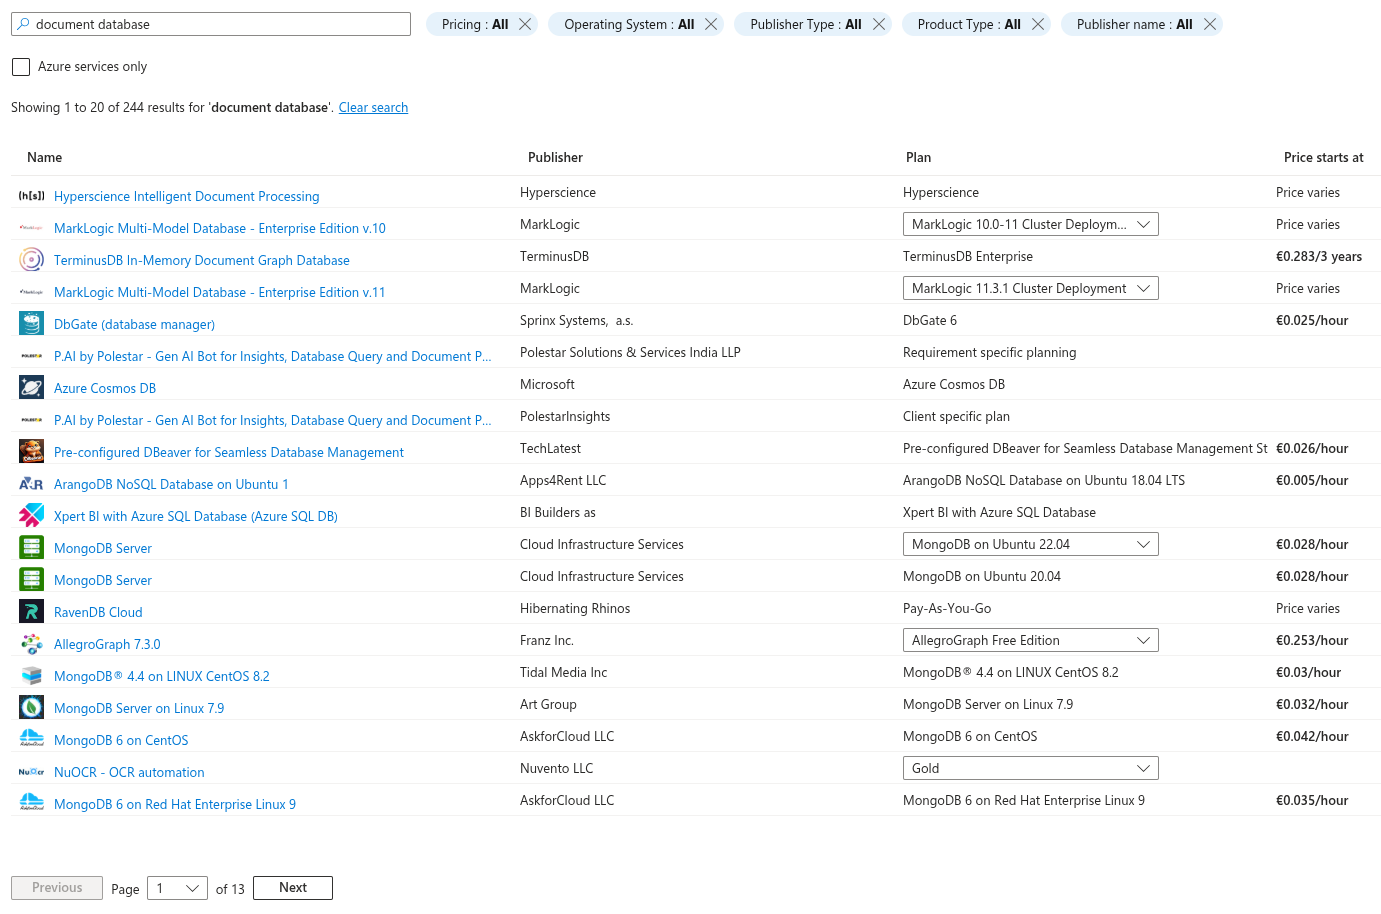
\includegraphics[width=\textwidth]{AzureDatabase.png}
    \caption{Proposte di Azure per i database documentali}
\end{figure}


\begin{wrapfigure}{r}{0.25\textwidth}
    \centering
    
\includegraphics[height=.12\textheight]{cosmos.png}
    Azure Cosmos
\end{wrapfigure}
Pur essendo focalizzato sui database documentali,
Cosmos DB è però una soluzione multi-modello e multi-API.
Supporta infatti, oltre alla sua API nativa per NoSQL (che usa il modello a documenti JSON),
anche API compatibili con MongoDB, Apache Cassandra, Apache Gremlin (per i grafi) e Azure Table.
Questa versatilità permette agli sviluppatori di utilizzare strumenti familiari,
semplificando la migrazione di applicazioni esistenti o
lo sviluppo di nuove con la flessibilità di scegliere il modello di dati più appropriato.\\
\\
A livello di costi è difficile portare un'analisi precisa,
in quanto tutti i competitor presentano servizi
con capacità, disponibilità e intregrazione differenti.
I modelli di pagamento che utilizzano metriche di utilizzo diverse,
rendendo necessarie ulteriori analisi che dipendono anche
dall'effettiva tipologia e quantità delle richieste che vertono sul database.
Di seguito viene riportata una tabella per comparazione i costi delle alternative principali.
Cosmos usa come metrica le Rerquest Units(RU) per quantificare l'impatto di una richiesta sul database.
Le RU rappresentano un'astrazione delle risorse di sistema (CPU, I/O, memoria).
Ogni operazione consuma RU, proporzionalmente alla sua
complessità, dimensione e al carico computazionale richiesto.\\

\begin{longtable}{|P{3.2cm}|P{4.2cm}|P{4.2cm}|P{3cm}|}
    \hline
    \textbf{Servizio}      & \textbf{Costo ogni milione di scritture}\newline(normalizzate a 1 KB) & \textbf{Costo ogni milione di scritture}\newline (normalizzate a 1 KB) & \textbf{Costo di manutenzione GB/mese} \\
    \hline
    AWS DynamoDB           & \$1.25                                                                & \$0.25                                                                 & \$0.25                                 \\
    \hline
    Google Cloud Firestore & \$0.90                                                                & \$0.30                                                                 & \$0.156                                \\
    \hline
    Azure Cosmos DB        & In base al consumo di RU, \$5.84 al mese ogni 100RU/s                 & In base al consumo di RU, \$5.84 al mese ogni 100RU/s                  & \$0.25 (Transazionale)                 \\
    \hline
    \caption{Costi dei principali database documentali gestiti in Cloud}
\end{longtable}

La difficoltà di stabilirne il costo in una fase iniziale
è mitigata però dalla presenza di un piano gratuito perenne.
Cosmos DB offre infatti una quota gratuita di risorse iniziali,
per tutta la durata dell'utilizzo.
Il piano prevede 25 GigaByte di memoria gratuita,
a cui si aggiungono 1000 RU/s offerti per ogni categoria di operazione, 
suddivise in lettura, scrittura e eliminazione. 
Dato lo stadio iniziale del progetto queste caratteristiche sono state considerate sufficenti,
permettendo di sfruttare e testare le capacità di distribuzione.
Nel caso in cui, sfruttando dati derivati dall'utilizzo effettivo dell'applicazione,
un'analisi condotta durante fasi successive del progetto faccia emergere che 
Cosmos DB non rappresenti l’opzione più adeguata, 
lo spostamento dei dati verso un altro gestore comporterà uno sforzo limitato,
data la compatibilità nella rappresentazione dei dati tra le diverse tecnologie di database documentali.

\subsection{La configurazione di Cosmos DB}

La creazione di una nuova istanza di Cosmos DB
richiede la definizione delle impostazioni di funzionamento,
che ne determinano le proprietà, a livello di disponibilità, ridondanza, sicurezza e resilienza ai guasti.\\
\\
La prima impostazione riguarda la distribuzione geografica dei dati.
Cosmos distribuisce sue risorse in zone, che vengono raggruppate in regioni.
L'opzione di usare delle availability zones duplica i dati su più zone all'interno della stessa regione.
Questo crea ridondanza dei dati per una maggiore resistenza ai guasti,
e così facendo aumenta la disponibilità dei dati, 
che da un disponibilità garantita iniziale per la zona singola del 99.99\% (sulle scritture) sale al 99.995\%,
evitando la perdita dei dati e delle funzionalità in caso una zona non sia più raggiungibile.
L'aggiunta di ulteriori regioni diminuirebbe il rischio indisponibilità a causa di guasti
(i dati verrebbero duplicati anche tra le varie regioni),
ma aumenterebbe la complessità e il costo dell'applicazione.
Per una fase iniziale si è optato per garantire una ridondanza a livello di zone,
selezionando quindi l'opzione delle availability zones, 
rimanendo però all'interno di una regione singola.\\

\begin{figure}[h!]
    \centering
    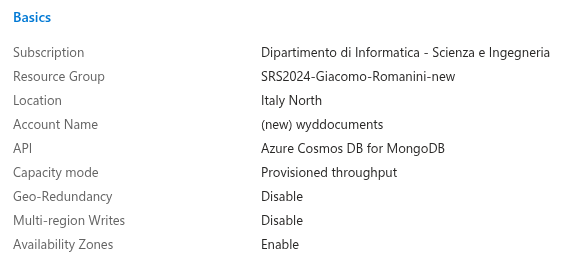
\includegraphics[width=\textwidth]{cosmosbasics.png}
    \caption{Impostazioni generali di Azure Cosmos DB}
\end{figure}

Volendo inizialmente rimanere in una singola regione,
l'impostazione "Geo-Redundancy" non è stata abilitata.
Allo stesso modo le scritture su più regioni non sono state abilitate,
preferendo un approccio centralizzato.\\
\\
Come modello di costo Azure propone due modalità distinte: Serverless e Provisioned throughput.
Nella modalità serverless il servizio scala in base alle richieste,
e considerando quindi solo l'effettivo utilizzo di risorse richieste.
Adatto a carichi di richieste improvvisi e sbilanciati,
non supporta l'esecuzione su più regioni.
Il provisioned throughtput invece richiede una previsione delle risorse necessarie,
per metterle a disposizione e farsi pagare di conseguenza, che siano state usate o meno.
Questo necessita quindi di una stima del carico previsto,
per poi impostare le risorse.
Azure propone però un metodo chiamato autoscale, 
che permette di modificare automaticamente (all'interno di un intervallo predefinito)
le risorse messe a disposizione in base al carico del momento,
per poi considerare il massimo valore raggiunto in quell'ora.
Questo permette di evitare l'implementazione di una strategia,
mantenendo comunque i costi legati al consumo effettivo delle risorse.
Prevedendo un carico di richieste non troppo elevato,
ma anche costante e poco variegato, 
e considerando un tempo di latenza minore e il supporto a regioni multiple,
si è scelta una strategia di pagamento di tipologia Provisioned throughput,
che verrà poi impostata per scalare automaticamente in un intervallo di risorse inizialmente contenuto.\\
\\
Per migliorare la sicurezza del database e garantire il controllo degli accessi
il database è stato inserito all'interno di una rete virtuale privata,
limitando l'accesso ai soli altri nodi che ne fanno parte,
isolandolo verso l'esterno.
Verranno quindi aggiunti alla rete solo i servizi che devono comunicare con Cosmos DB,
in particolare Azure Functions e il KeyVault(che contiene le chiavi per la cifratura dei dati).
Nonostante la ridondanza nelle zone garantisca il ritrovamento dei dati 
anche in caso di indisponibilità di un'istanza del database,
si è scoperti qualora avvengano modifiche erronee o malintenzionate.
Il servizio di backup proposto da Azure permette di salvare lo stato dei dati 
fino a un certo momento nel passato, 
in maniera tale garantire il ritorno a una situazione precedente 
in caso ci si accorga siano avvenute modifiche non desiderate. 
Azure permette sia di personalizzare la tipologia di backup,
in termini di durata, grandezza dei salvataggi e numero di copie,
sia di seguire delle opzioni già configurate.
Nel nostro caso si è scelto di applicare il servizio incluso gratuitamente
che mantiene le modifiche avvenute negli ultimi sette giorni.\\
\\

\clearpage



\subsection{La definizione delle classi}


bisogna definire le classi in maniera da sfruttare la maniera di archiviazione 
per ottimizzare il carichi delle richieste previsti.
essendo la memoria in un database relazionale abbiamo ampia libertà di modellazione delle entità.
 ogni principale entità (a parte per gli account) sono stati definite delle collezioni.
laddove possibile, sono state incluse le relazioni all'interno di un solo documento,
quali evento immagini, gli account con gli utenti, e la relazione utenti-profili(roles).
i profili e gli eventi descrivono solo le informazioni essenziali per il loro recupero
La relazione tra gruppi e profili è descritta da groups e profile details, duplicati
 aggiunto anche per salvare tutte le impostazioni che interessano solo il profilo stesso.
 è stato creato event details per separare le informazioni essenziali
 per le query di recupero da quelle di dettaglio.\\
 \\
la relazione centrale del progetto tra event e profile è stata 
duplicata in due documenti: ProfileEvent e EventProfile.
EventProfile è salvato con event e copre la necessità di poter visualizzare i profili che hanno confermato l'evento.
partition key, sono separati dall'evento in maniera tale da permettere 
la conferma simultanea allo stesso evento da parte di più profili.
ProfileEvent serve invece a recuperare gli eventi associati al profilo, 
eventulmente analizzando anche la data di aggiornamento.

roles\\
\\


\begin{figure}[h!]
    \centering
    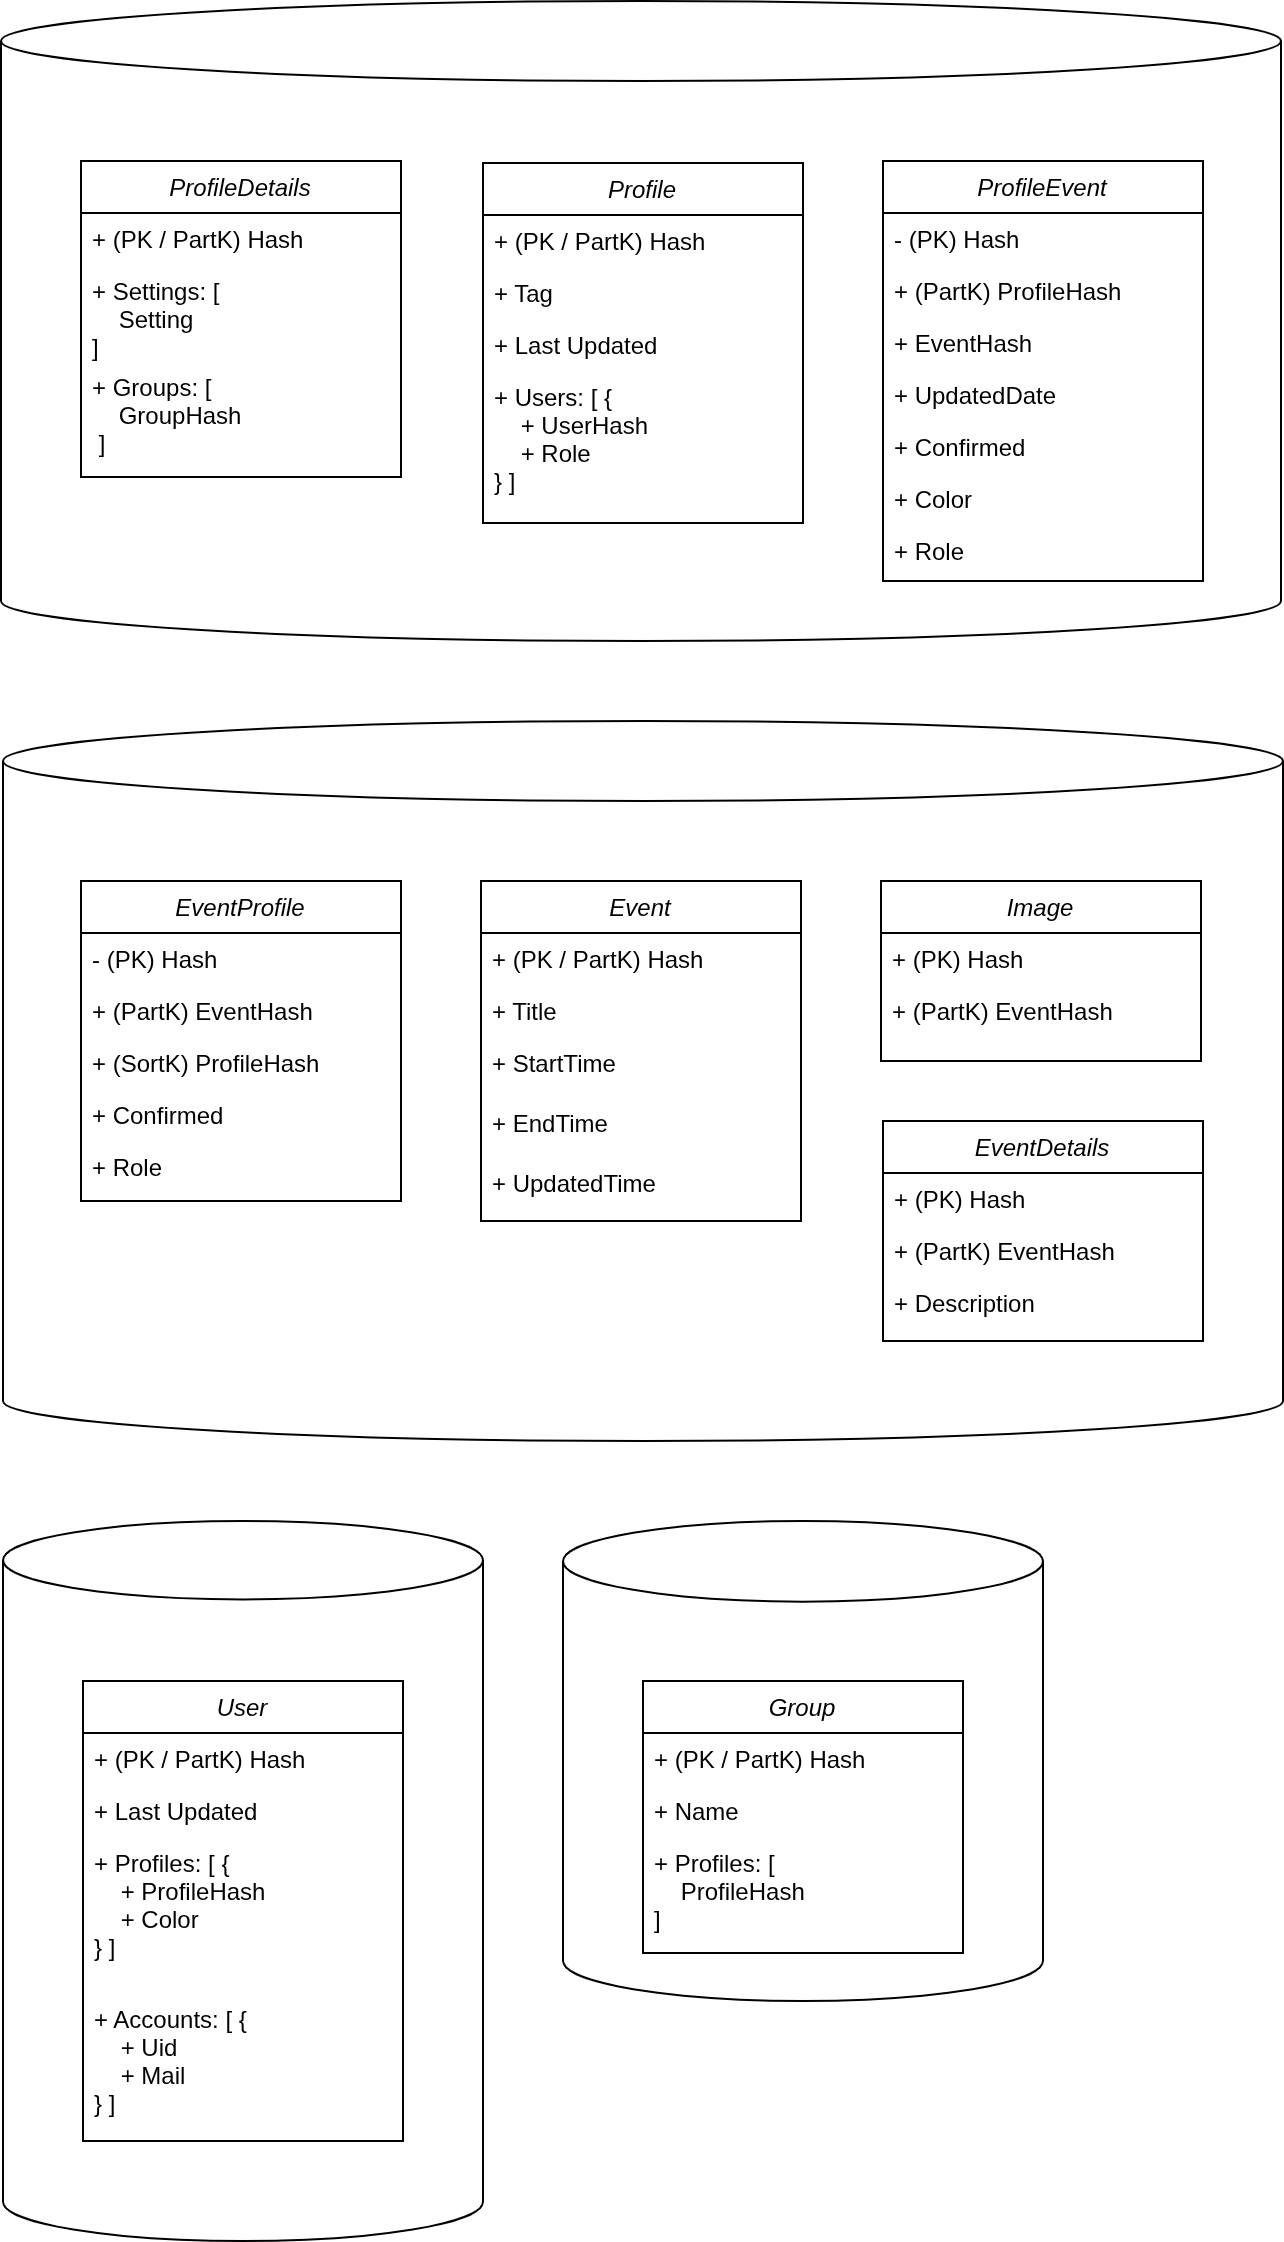
\includegraphics[width=\textwidth]{NonRelazionalModel.png}
    \caption{Modello delle collezioni}
\end{figure}

Nonostante sia più probabile che venga richiesto il dettaglio di un evento,
e quindi sia più frequente il dover recuperare i Profile relativi all’Event,
la proporzione delle richieste prevista non giustifica lo sbilanciamento della relazione sugli Event.
Infatti, se si salvassero tutti i ProfileEvent sull’oggetto Event,
le richieste degli eventi appartenenti ai profili, sebbene meno frequenti,
richiederebbero l’ispezione di tutti gli Event alla ricerca del Profile indicato.
Infine, se si duplicasse l’oggetto ProfileEvent,
oltre che nella sua tabella originaria, anche sugli Event la sua creazione,
la sua eliminazione e la modifica del campo Confirmed richiederebbero il doppio delle scritture.\\
\\



\subsection{L'integrazione con le Azure Functions: il framework .Net e l'eventual consistency}

\clearpage




\clearpage




\subsection{L' integrazione con Le azure functions}

La scelta di un database relazionale per la persistenza ha comportato sviluppi progettuali precisi.
In primis si rende necessario tradurre il dominio in componenti relazionali che possano essere espressi e salvati nelle tabelle del database.

var cosmosClient = new CosmosClient("<your-connection-string>");

per il collegamento da remoto, è necessario utilizzare una VPN per connettersi alla virtual Network

\begin{figure}[h!]
    \centering
    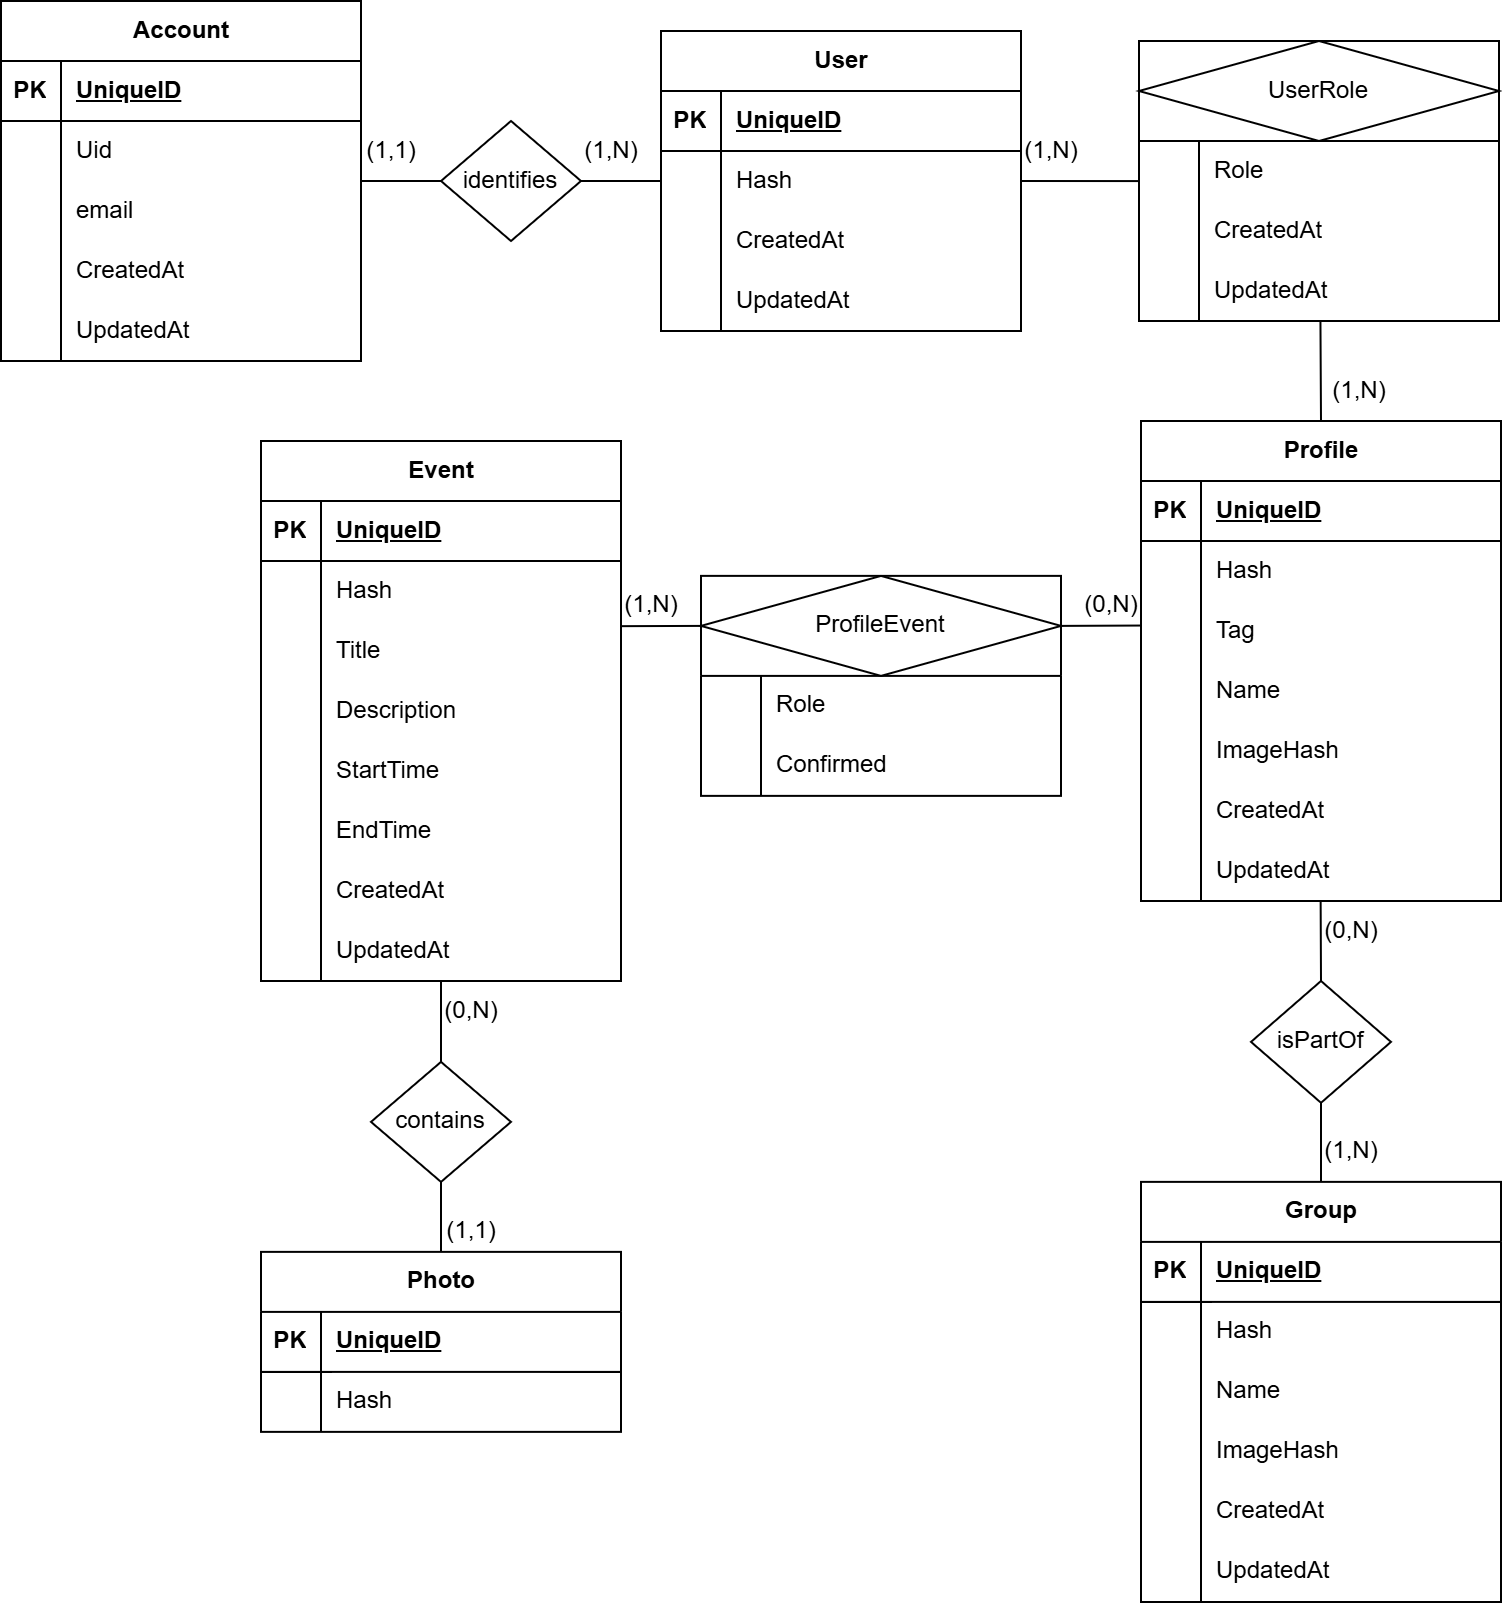
\includegraphics[width=\textwidth]{ProgettoDiagrammaER.png}
    \caption{Diagramma Entità - Relzione del dominio}
\end{figure}

Si creano quindi sul server le classi logiche del programma, a partire dal dominio.
Ogni classe corrisponde ad un oggetto del dominio, presentando i valori e le relazioni dei componenti come attributi dell’oggetto.\\
\\
Entity Framework Core di .Net(EFCore) è una libreria di C\# che permette di unire le classi logiche del programma alle tabelle del database.
Fornisce un’astrazione logica del collegamento con il database e le richieste relative, fornendo una rappresentazione di alto livello delle connessioni sottostanti. \\
\\
Una volta collegato il server con il database tramite le stringhe di connessione salvate sull’Azure Key Vault,
sono state definite le proprietà tra le varie entità, per poi inizializzare in automatico la struttura del database.
Le modifiche alla struttura del database vengono infatti generate automaticamente da EFCore in seguito alla creazione o alla modifica degli attributi degli oggetti.
Questo permette di star dietro agli aggiornamenti, generando e salvando le modifiche da applicare ad ogni modifica delle proprietà del dominio.\\
\\
\begin{figure}[h!]
    \begin{center}
        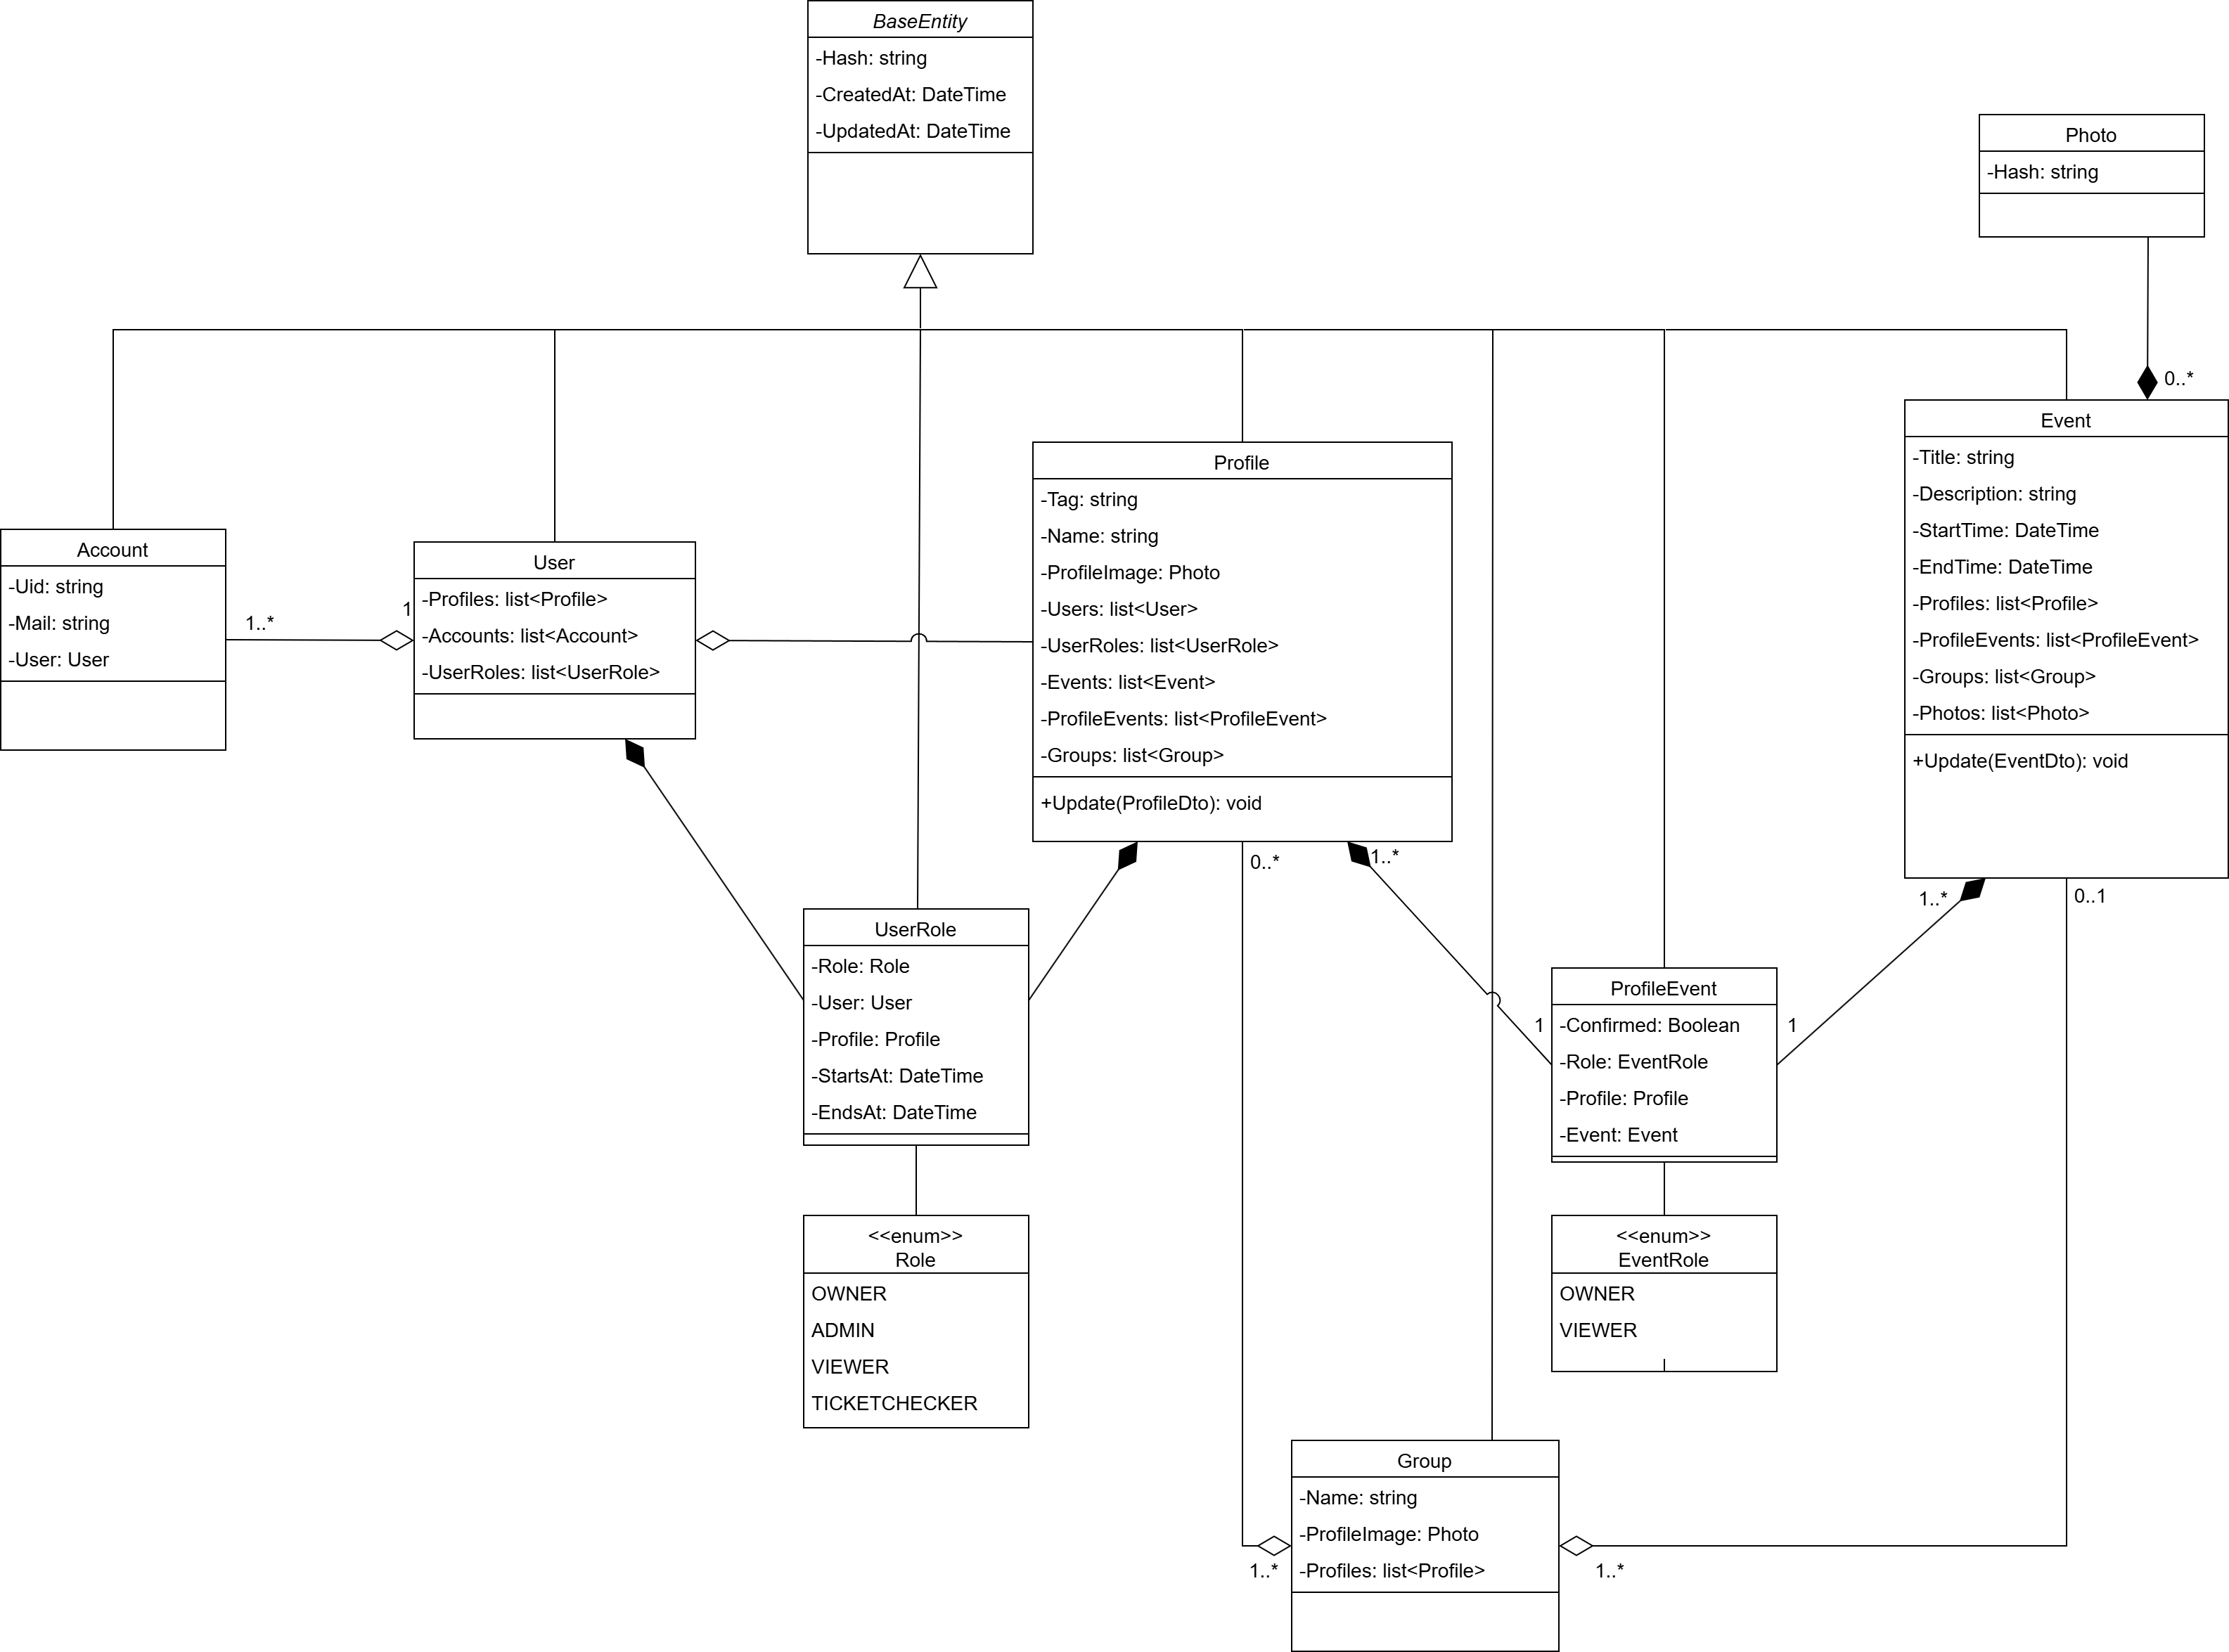
\includegraphics[width=\textwidth]{ModelClassDiagram.png}
        \caption{Modello delle classi del client}
    \end{center}
\end{figure}

Per la riduzione del carico computazionale richiesto da elementi con tante relazioni si utilizza la tecnica del lazy loading.
La tecnica del Lazy Loading consiste nel richiedere i dati delle relazioni di un elemento solo quando strettamente necessario.
La sua realizzazione tramite EFCore è attuata grazie alla proprietà virtual,
che permette di gestire un oggetto con un riferimento al database richiedendo i dati delle sue relazioni solo quando viene espressamente richiesto.\\
\\


Inoltre, Azure mette a disposizione molteplici servizi accessori che possono essere uniti al servizio.
Questo permette di estendere le potenzialità del database tramite  l’analisi e il monitoraggio dei dati,
generando prestazioni aggiuntive o integrando i dati per lo sviluppo di altre tecnologie.\\
\\

Al server principale è stata affiancata una replica che rimane costantemente aggiornata.
Situata in una località differente dal server principale,
garantisce alta disponibilità continuando a fornire i servizi anche in caso di malfunzionamenti al server principale.\\
\\

Nel caso in cui però fossero necessarie ulteriori prestazioni,
se il dominio e i requisiti lo permettono,
si può eventualmente delegare a un database non relazionale le modifiche ai dati e alle relazioni
che non necessitano delle qualità ACID ma richiedono un’alta frequenza di scrittura.\\
\\
Interporre una cache tra la logica applicativa e il database
semplifica e riduce il numero di richieste verso il database.
Il livello di caching si occupa di gestire le richieste al database
fornendo e duplicando le risposte che possiede già in memoria,
eventualmente concentrando le richieste in caso i dati siano invece da recuperare.
Per i dati in scrittura, invece, salva temporaneamente le modifiche richieste,
aggiornando subito la memoria locale,
per poi apportare le modifiche al database in momenti di carico ridotto.
Garantisce così un tempo di risposta e di propagazione degli aggiornamenti ridotto,
alleviando il numero di richieste al database, estendendo così  le prestazioni fornite.\\
\\


Tuttavia, non vi è alcun vincolo che impedisca l'affiancamento di database di tipologia diversa
per rispondere a esigenze specifiche e sfruttare i punti di forza di entrambe le tecnologie.
\\
\clearpage